% Dataset and EDA, with the feature-group ablation
% Refers to tab:clip and tab:features from the Methodology section.

\section{Dataset and Exploratory Analysis}

\subsection{Dataset}
We use the Next Day Wildfire Spread dataset~\cite{huot2022}: 18\,545 samples of active fires across
the contiguous United States from 2012 to 2020. Each sample is a $64\times64$\,km patch at 1\,km
resolution with 12 input channels on day $t$ (elevation from SRTM; wind direction and speed, minimum
and maximum temperature, specific humidity, precipitation and ERC from GRIDMET; the Palmer drought
index from GRIDMET Drought; NDVI from VIIRS; population density from GPWv4; and the MODIS active-fire
mask) and the MODIS fire mask on day $t+1$ as the label. Fires more than 10\,km apart are treated as
separate events, and every sample contains fire on day $t$. Calendar weeks are assigned at random
to train, eval and test in an 8:1:1 ratio with a one-day buffer, giving 14\,979 / 1\,877 / 1\,689 patches.

\subsection{Labels and class imbalance}
Fire masks use three values: fire (1), no fire (0) and uncertain ($-1$, e.g.\ cloud or smoke).
Uncertain pixels make up 1.1--1.4\% of day-$t$ masks and 2.3--2.8\% of day-$t{+}1$ masks, with
similar shares in every split, so ignoring them in training and evaluation introduces no shift
between splits. Next-day fire covers only 1.10\% of labelled training pixels (90:1), 1.37\% on eval
and 1.25\% on test; an all-zero predictor would exceed 98.7\% accuracy, which is why we report
PR AUC. Across the 14\,979 training patches, 58.2\% of fires grow from day $t$ to $t+1$, 38.7\% shrink and 3.1\% keep
the same size (Fig.~\ref{fig:growth}), matching the 58\%/39\% reported by Huot et al.
Shrinking fires make persistence over-predict, and many small day-$t$ fires gain far more pixels
on day $t+1$.

\begin{figure}[t]
\centering
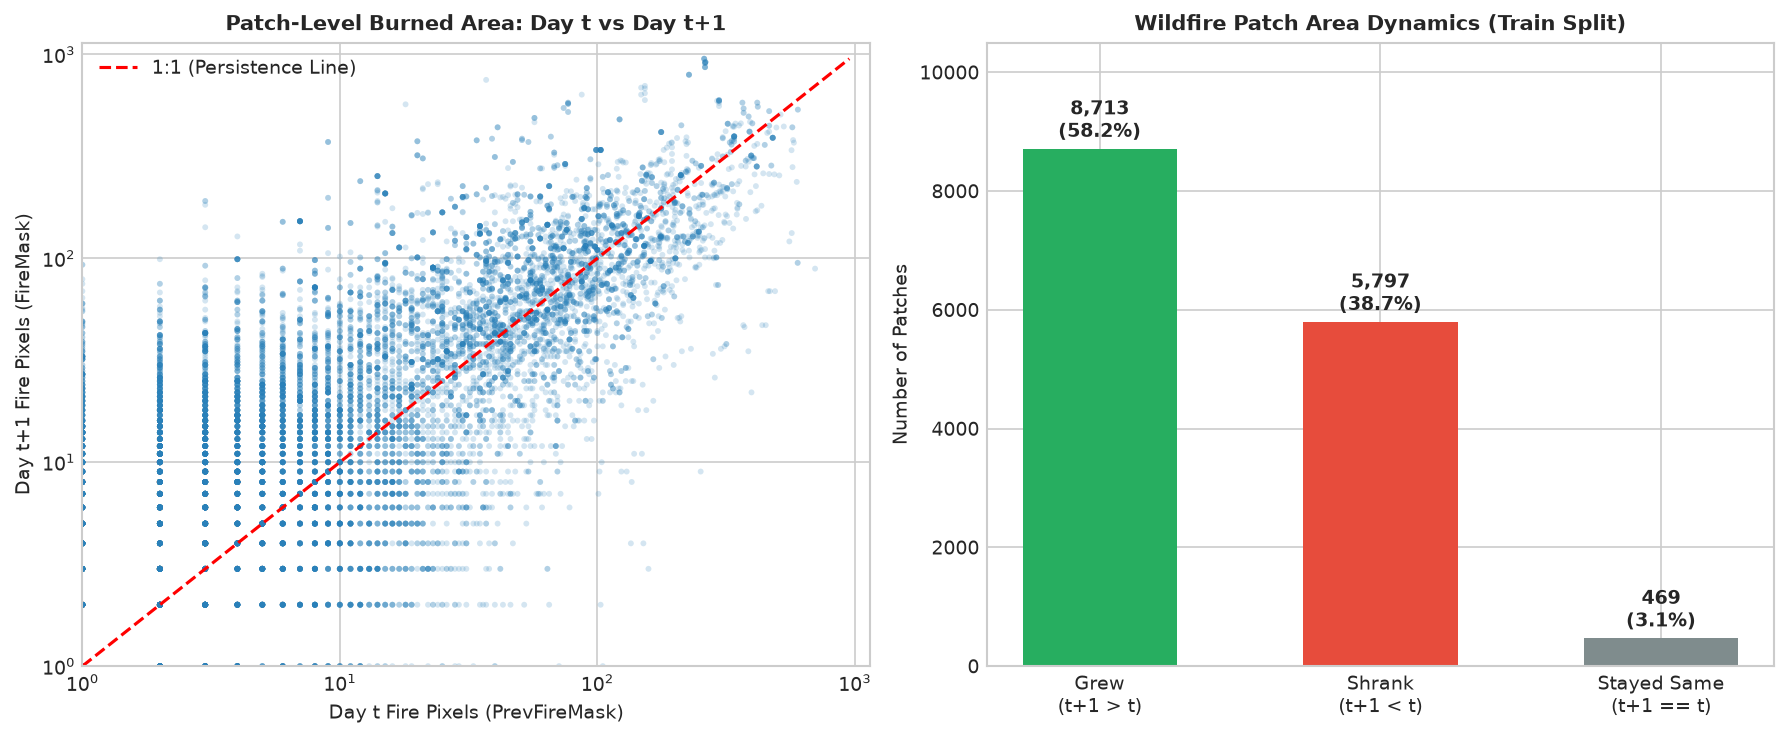
\includegraphics[width=\columnwidth]{figures/eda_patch_fire_growth.png}
\caption{Burned area per training patch on day $t$ vs.\ day $t+1$ (left, log scale, dashed line =
persistence) and the share of patches that grow, shrink or stay the same (right).}
\label{fig:growth}
\end{figure}

\subsection{Data quality}
The raw export contains physically impossible values: wind direction outside $[0^\circ, 360^\circ]$
in 0.23\% of training pixels (from $-505\,870^\circ$ to $37\,736^\circ$), temperatures from $-445$\,K
to 1\,230\,K in 0.36\% of pixels, negative precipitation in 9.8\% of pixels, and a few negative
wind speed, humidity and ERC values. These are corrected as described in the Methodology section
(Table~\ref{tab:clip}). Negative elevation (down to $-45$\,m) and negative NDVI (water, snow) are
real and left unchanged. NDVI is stored multiplied by $10^4$.

\subsection{Channel relationships and marginal signal}
Minimum and maximum temperature are strongly correlated (Spearman $\rho = 0.89$), humidity follows
temperature ($\rho = 0.70$ with \texttt{tmmn}), and elevation correlates with ERC ($0.66$) and
negatively with humidity ($-0.48$) and population ($-0.47$). The day-$t$ fire mask has near-zero rank
correlation with every raw channel ($|\rho| \le 0.09$). Comparing next-day fire and no-fire pixels
(balanced sample, Fig.~\ref{fig:fire_vs_nofire}), ERC (median 75 vs.\ 54) and elevation (1\,414 vs.\
709\,m) separate the classes most clearly, maximum temperature and NDVI shift slightly (28.0 vs.\
26.8\,$^\circ$C; 0.51 vs.\ 0.55), and wind speed and specific humidity barely differ at the median.

\begin{figure}[t]
\centering
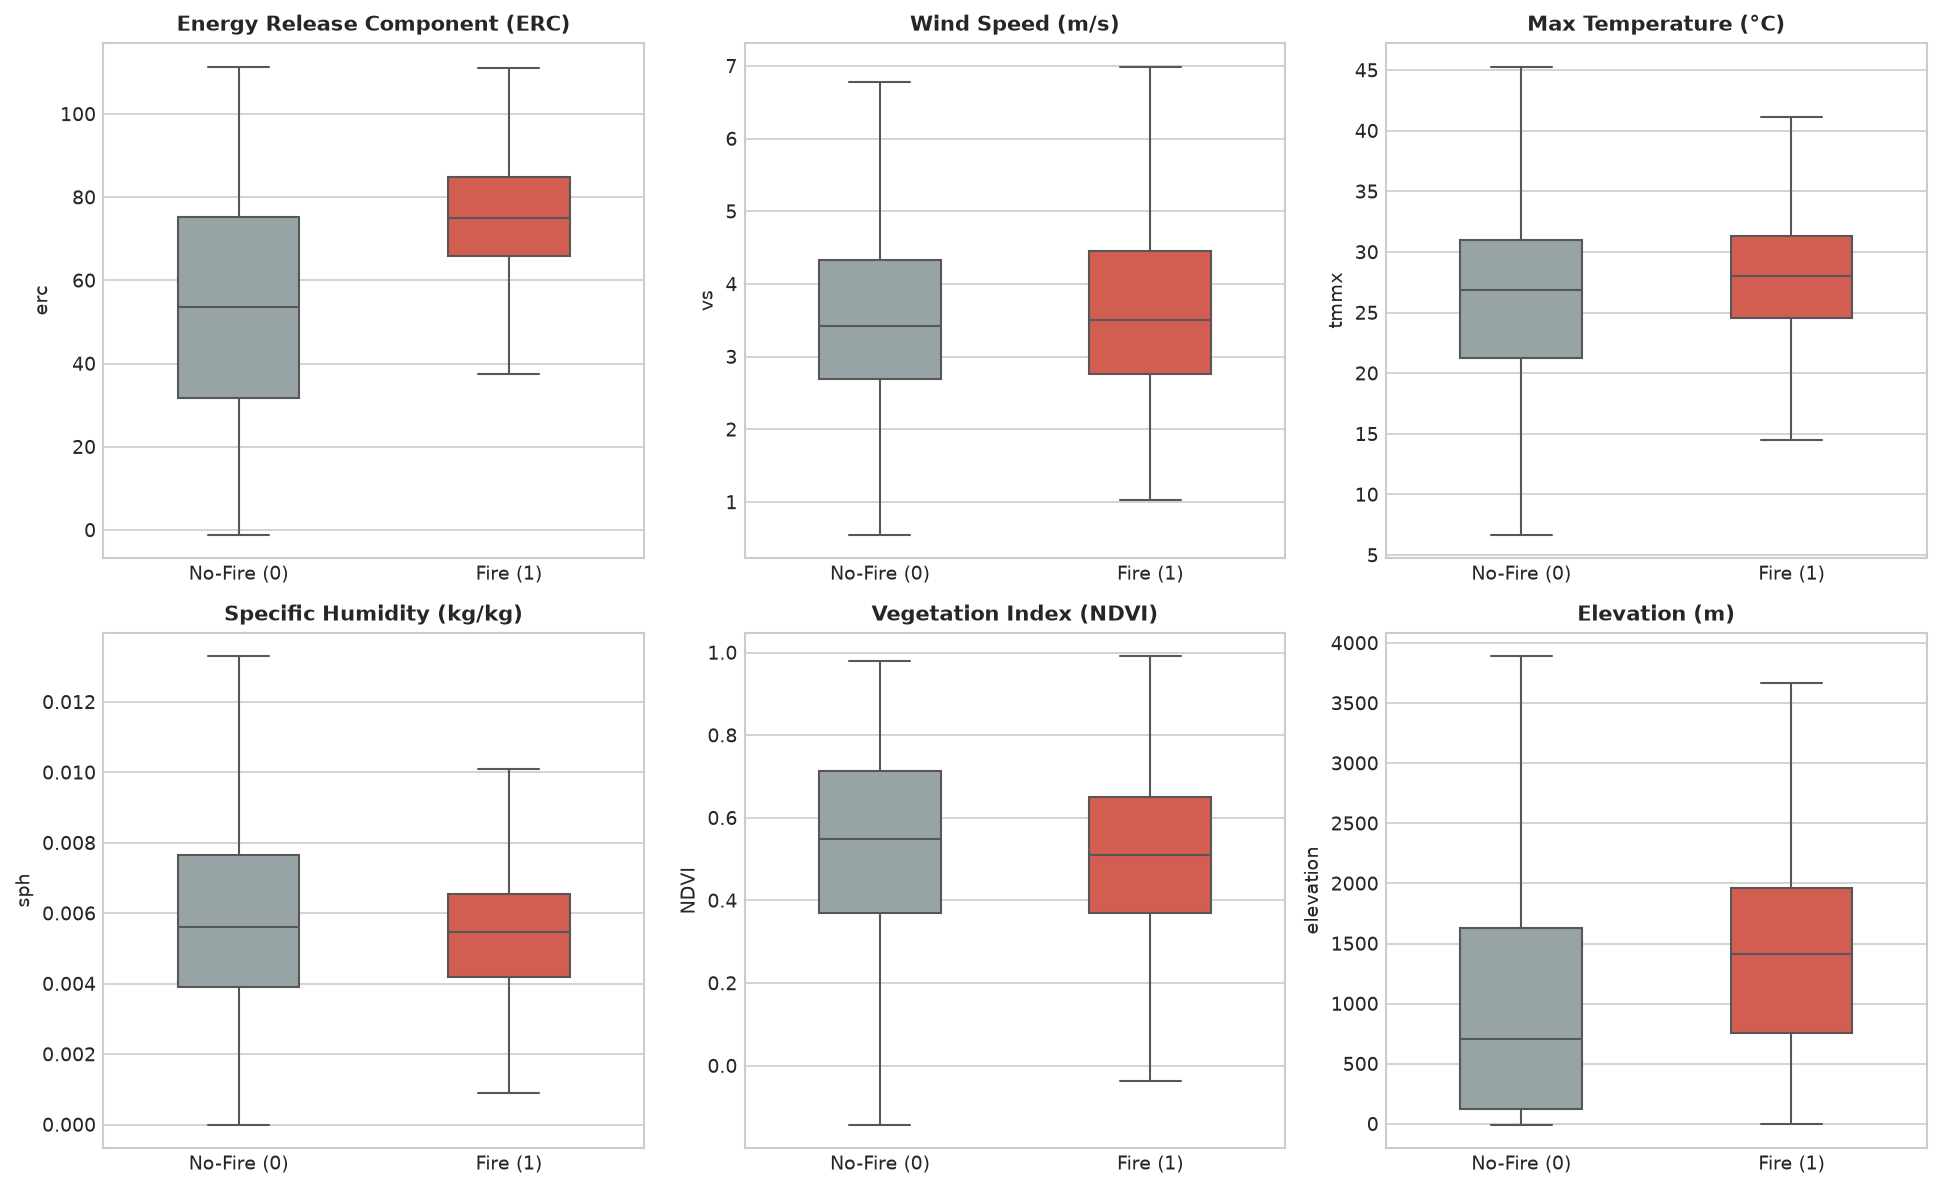
\includegraphics[width=\columnwidth]{figures/eda_fire_vs_nofire_features.png}
\caption{Raw channel distributions for next-day fire vs.\ no-fire pixels (balanced 50k/50k training
sample, outliers hidden).}
\label{fig:fire_vs_nofire}
\end{figure}

\subsection{From EDA to features}
Three findings shaped the pipeline. (i) A pixel's own weather says little about whether it burns,
while burning depends strongly on nearby fire, so most engineered features describe the fire
neighbourhood (Table~\ref{tab:features}). (ii) Measuring each next-day fire pixel's distance to the
nearest day-$t$ fire shows that 40.4\% lie more than 5\,km away and 26.1\% more than 10\,km away;
we therefore added an upwind fire feature at 8\,km (\texttt{upwind\_fire\_k8}), which ranks 5th of
35 features by gain in the tuned XGBoost. (iii) Wind direction is circular, so out-of-range values
are wrapped rather than clipped. We did not clip negative NDVI, because water and snow are genuine,
informative non-fuel.

\subsection{Feature-group ablation}
To measure what each feature group contributes, we retrain the tuned LightGBM with identical
hyperparameters while removing one group at a time, plus a run with the fire-neighbourhood group
only (Table~\ref{tab:ablation}, Fig.~\ref{fig:ablation}). Each run chooses its F1 threshold on eval
and is scored on test. Removing the fire-neighbourhood features collapses PR AUC from 0.248 to 0.048,
mirroring Huot et al., where removing the previous fire mask cuts PR AUC from 28.4\% to 6.8\%.
Among the environmental groups, vegetation matters most ($-0.009$), again in line with Huot et al.,
who found vegetation the most useful variable alongside the fire mask. Removing weather costs only
0.001, and removing terrain or population changes PR AUC by $+0.003$ and $+0.002$; differences this
small are within run-to-run noise and suggest these groups overlap with the remaining features.
The fire-neighbourhood features alone reach 0.218, so the environmental variables add 0.031
(14\%) on top of fire location. Because the upwind and alignment features use wind direction,
the ``no weather'' run still sees some wind information.

\begin{table}[t]
\centering
\caption{Feature-group ablation (LightGBM, test split, F1 at eval-chosen threshold).}
\label{tab:ablation}
\begin{tabular}{lrrrr}
\hline
Run & \#feat. & PR AUC & $\Delta$ & F1 \\
\hline
All features & 35 & 0.248 & -- & 0.331 \\
No weather & 21 & 0.248 & $-0.001$ & 0.334 \\
No vegetation & 31 & 0.240 & $-0.009$ & 0.333 \\
No terrain & 30 & 0.251 & $+0.003$ & 0.340 \\
No fire neighbourhood & 25 & 0.048 & $-0.200$ & 0.093 \\
No human & 33 & 0.251 & $+0.002$ & 0.336 \\
Fire neighbourhood only & 10 & 0.218 & $-0.031$ & 0.334 \\
\hline
\end{tabular}
\end{table}

\begin{figure}[t]
\centering
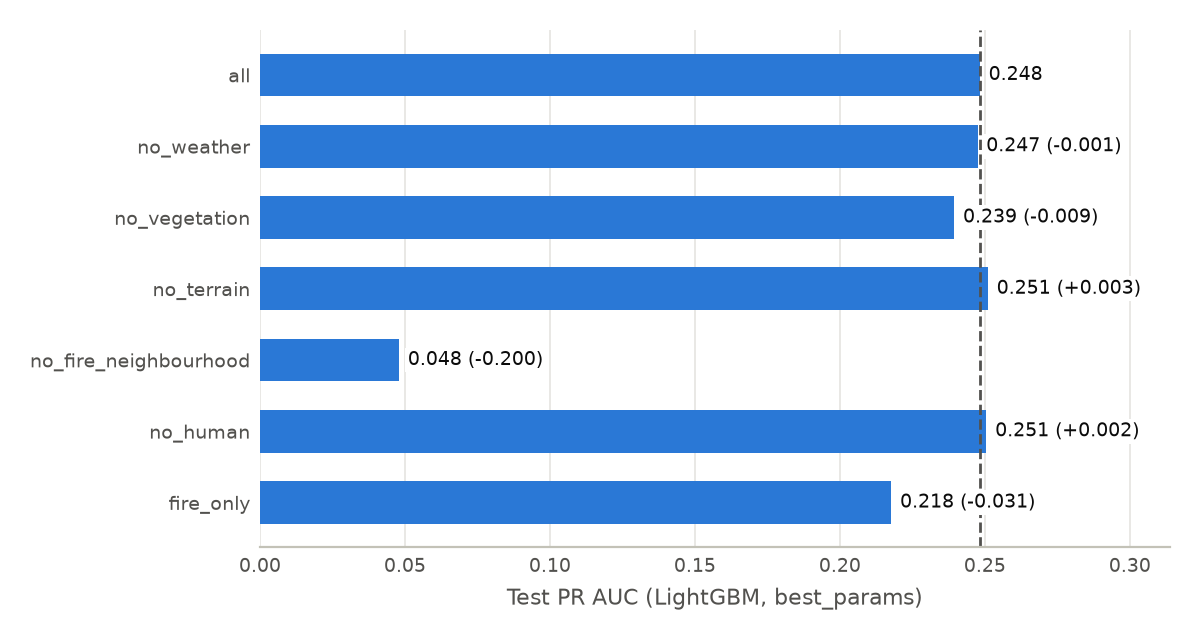
\includegraphics[width=\columnwidth]{figures/ablation_pr_auc.png}
\caption{Test PR AUC per ablation run; the dashed line marks the model with all features.}
\label{fig:ablation}
\end{figure}
